\chapter{Desarrollo de software confiable}

\section{Introducción}
En este apartado se describe el procedimiento seguido hasta conseguir implementar TEE. Al principio se hace uso de la tarjeta Zedboard de Xilinx. Sin embargo, surgen varios inconvenientes a medida que avanza el trabajo, que sumados a algunos requisitos del trabajo provocan que se deba cambiar de dispositivo. El dispositivo que se acaba usando es una Raspberry Pi 3. \newline

El procedimiento seguido para desarrollar una aplicación de ejemplo sobre TrustZone en Zedboard resulta muy representativa de lo que se consigue con esta tecnología de ARM. Se incluye dicho procedimiento de manera detallada ya que en Raspberry Pi se hace uso del proyecto OP-TEE que realiza el procedimiento de manera transparente.

\section{ARM TrustZone en Zedboard}

El primer dispositivo sobre el que se pretende desarrollar un diseño con TrustZone habilitado es la tarjeta Zedboard de Xilinx. La información práctica existente proporcionada por ARM o Xilinx de manera abierta sobre TrustZone es muy reducida. La documentación que proporcionan trata de manera teórica el tema, sin embargo, las guías y tutoriales prácticos (principalmente los de ARM) son de pago o bajo acuerdos. Debido a esto, se propone en un primer momento realizar un diseño de ejemplo que sirva de aprendizaje y comprobación del correcto funcionamiento de TrustZone.

\subsection{Diseño TrustZone Hello World}
Para este diseño se hace uso del software \textit{Vivado Design Suite} de Xilinx. La principal guía de usuario proporcionada por Xilinx se titula \textit{Programming ARM TrustZone Architecture on the Xilinx Zynq-7000 All Programmable SoC} \cite{guiaxilinx}. En esta guía aparecen reflejados los cambios y configuración necesarios en registros, señales, memoria, etc. A su vez se hace uso de un tutorial \cite{vivadotutorial} que se basa en la guía de Xilinx. Esta documentación es la base para desarrollar el diseño de ejemplo.\newline

El diseño consiste en configurar como seguro un GPIO y desarrollar dos aplicaciones \textit{Hello World} (una en el Mundo Seguro y otra en el Mundo Normal) que se llamen una serie de veces la una a la otra mediante el Monitor.\newline

Los primeros pasos a seguir son los convencionales, se crea un proyecto para la tarjeta Zedboard y se crea el diseño de bloques deseado. En este caso consiste del Sistema de Procesamiento ZYNQ, 3 GPIOs y los correspondientes bloques (como el AXI de Interconexión) que se crean cuando se realiza la conexión automática de ayuda de Vivado. En la figura XXXXX se observa el diseño final. \newline

\begin{figure}
	\centering
	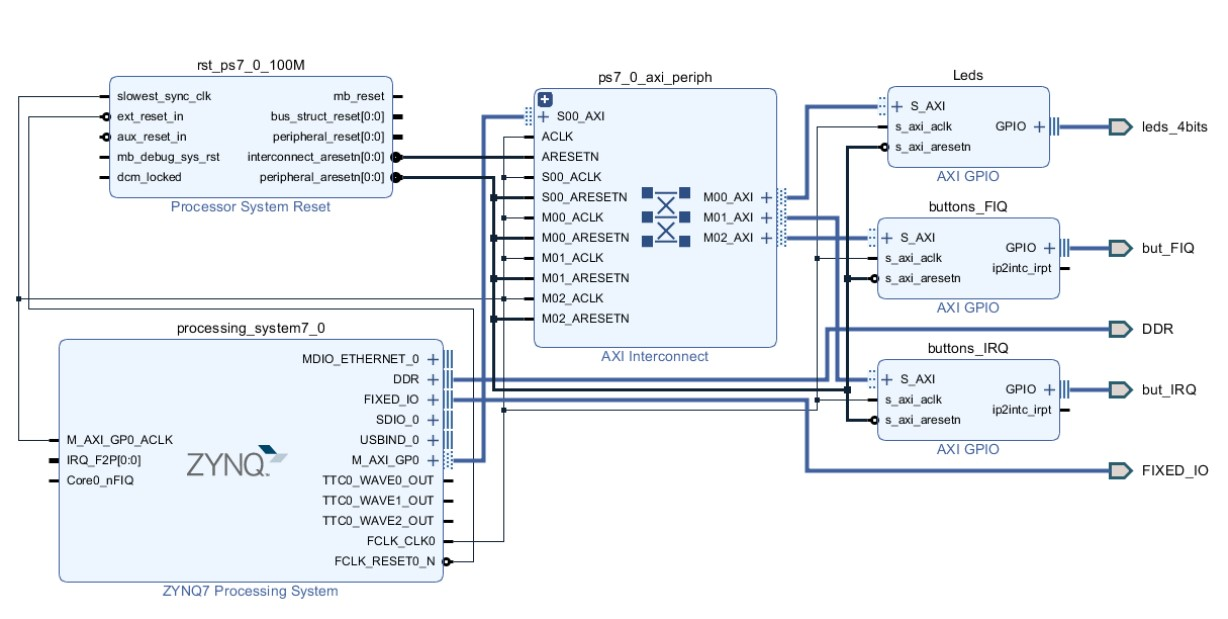
\includegraphics[width=1\textwidth]{imagenes/blockdesign.jpg}
	\caption{\label{fig1}Diseño de bloques final.}
\end{figure}

\subsubsection{Configuración del diseño}

En el diseño se configuran dos aspectos relevantes para TrustZone:

\paragraph{Interrupciones IRQ y FIQ.}
Como aparece descrito en la guía de usuario de Xilinx \cite{guiaxilinx} en el apartado \textit{Securing Interrupts}, el controlador de interrupciones del ARM Cortex A9-MP permite definir individualmente las interrupciones como seguras o no seguras. Las interrupciones no seguras se suelen señalizar haciendo uso del mecanismo de interrupciones IRQ. En cambio, las interrupciones seguras pueden utilizar tanto el mecanismo IRQ como el FIQ. En la configuración del procesador, en el apartado interrupciones, aparece la opción de habilitar tanto IRQ como FIQ. Una vez se habilitan como se observa en la figuraXXXXXXXXXX, ambas deben aparecer en el bloque del procesador para poder ser conectadas (se observan en la figura XXXXXXanterior). \newline


\begin{figure}
	\centering
	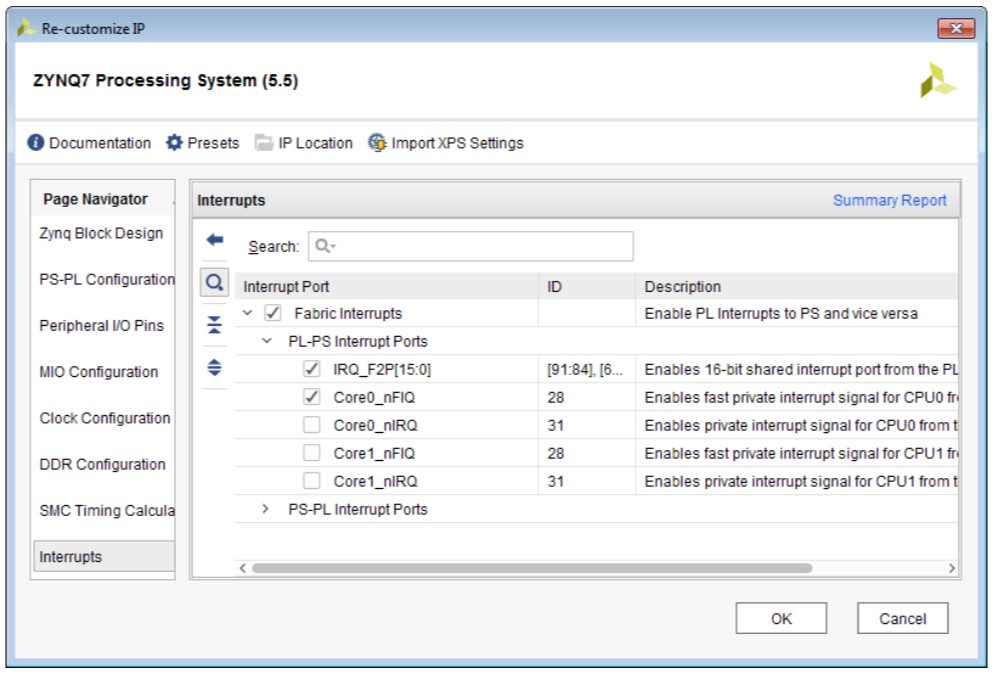
\includegraphics[width=1\textwidth]{imagenes/interrupciones.jpg}
	\caption{\label{fig1}Habilitar interrupciones IRQ y FIQ.}
\end{figure}

\paragraph{Securizar periféricos.}
En el diseño, M0X\_AXI es el máster que controla los periféricos (GPIOs). Para conseguir que uno de esos periféricos sea seguro hay que habilitar la opción \textit{Secure Slave} del bus encargado de la comunicación entre el \textit{AXI Interconnect} y el periférico en cuestión. En la configuración del  \textit{AXI Interconnect} en Opciones Avanzadas existe la posibilidad de configurar alguna de estas interfaces (M0X\_AXI) como seguras. En la figura XXXX se observa el procedimiento seguido para hacer segura la interfaz M00\_AXI encargada de controlar el GPIO denominado Leds. \newline

\begin{figure}
	\centering
	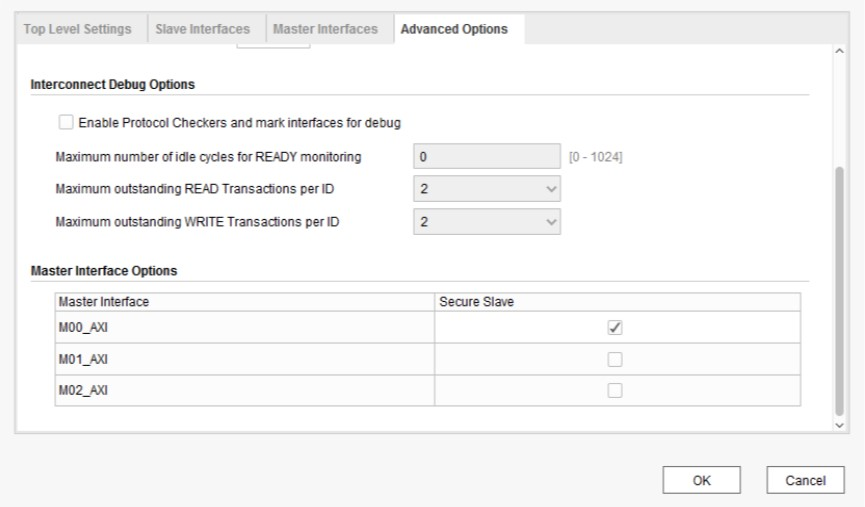
\includegraphics[width=1\textwidth]{imagenes/secureslave.jpg}
	\caption{\label{fig1}Securización de la interfaz del periférico.}
\end{figure}


\subsubsection{Implementación software}
Para esta tarea se hace uso del \textit{Software Development Kit} incluido en Vivado. Se exporta el proyecto al SDK para poder empezar a trabajar en él. \newline

Antes de poder comenzar a desarrollar el código de la aplicación de ejemplo, hay una serie de archivos del proyecto que hay que modificar e incluir algún otro para el correcto funcionamiento de TrustZone. Notar que estos archivos se encuentran tanto en el código ejemplo proporcionado por ARM \textit{Cortex-A9 TrustZone example} \cite{armexample}, como en el tutorial \cite{vivadotutorial}: \newline

\paragraph{Creación de proyectos.} Se pretender desarrollar una aplicación segura y otra no segura. Por lo tanto, será necesario crear dos proyectos que contentan una aplicación con la plantilla \textit{Hello World}.

\paragraph{Archivo \textit{lscript.ld}.} Estos archivos contienen las direcciones de las distintas regiones de memoria para cada aplicación. Se modifican tanto la dirección de origen como el tamaño de manera conveniente a cada aplicación. En el caso de la aplicación segura, hay que añadir una sección para la imagen de la aplicación no segura y la pila del monitor (consiste en dos particiones una para el Mundo Seguro y otra para el Mundo Normal).

\paragraph{Archivo \textit{monitor.S}.} Este archivo contiene la rutina para el \textit{Secure Monitor Call}. Su principal función es cambiar de un Mundo (Seguro/Normal) a otro, almacenando los registros de memoria del mundo en el que se encuentra y cargando los del mundo al que cambia.

\paragraph{Archivo \textit{normal.S}.} Este archivo es el encargado de enlazar con la imagen del Mundo Normal desde el Mundo Seguro. Esto es posible ya que se incluye el binario de la aplicación no segura en la aplicación segura.

\paragraph{Archivo \textit{platform.c.}} En este archivo se deben de incluir algunas líneas encargadas de (1) la definición de algunos macros para los registros TrustZone y (2) incluir la llamada a función de inicialización de TrustZone (\textit{init\_TZ()}) a la función \textit{init\_platform()}.

\paragraph{Archivo \textit{boot.S.}} Este archivo propio de Xilinx se encuentra en la ruta \textit{non\_secure\_bsp/ps7\_cortexa9\_0/libsrc/standalone\_v6\_2/src/}. Dicho archivo es un \textit{standalone} de Xilinx al que hay que realizar algunos cambios en la configuración del registro CP15 para que no se produzcan excepciones indeseadas.\newline

Una vez hecho esto se puede proceder a desarrollar el código de las aplicaciones (segura y no segura). Se parte de la plantilla existente para una aplicación de ejemplo Hello World. Se realizan una serie de cambios para que el comportamiento sea que una aplicación llame a la ejecución de la otra mediante llamadas al SMC. El código resultante se observa en las figuras XXXXXX y XXXXXXXXXXXXX.

\begin{figure}
	\centering
	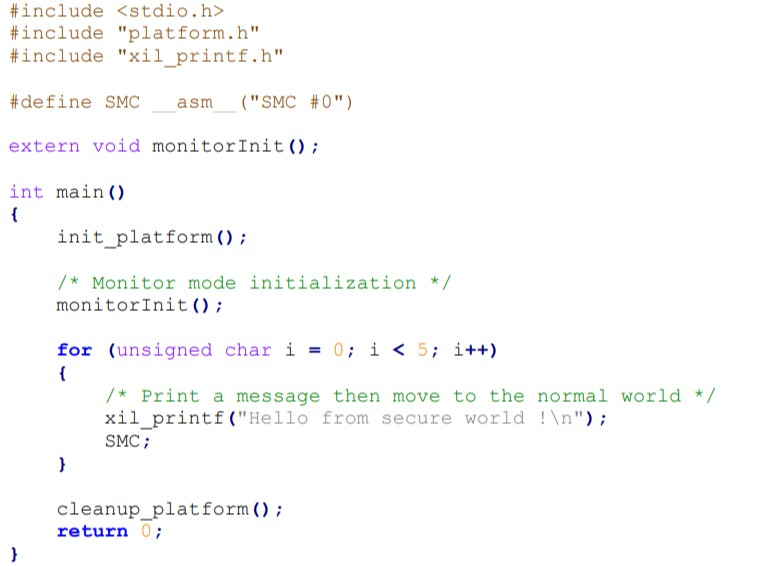
\includegraphics[width=1\textwidth]{imagenes/secureapp.jpg}
	\caption{\label{fig1}Código de la aplicación segura.}
\end{figure}

\begin{figure}
	\centering
	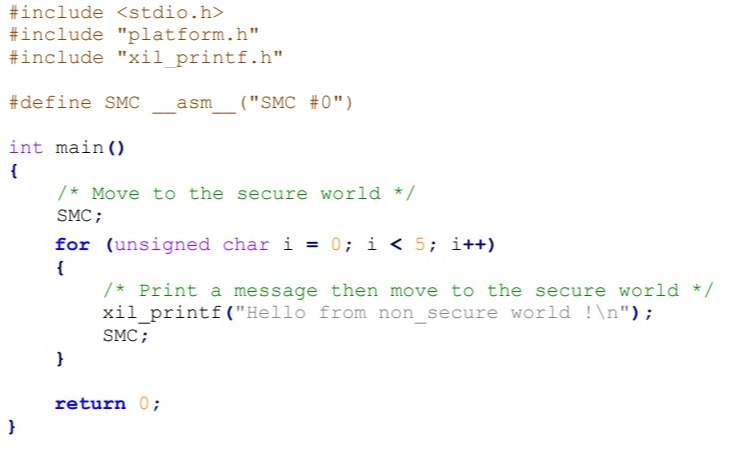
\includegraphics[width=1\textwidth]{imagenes/normalapp.jpg}
	\caption{\label{fig1}Código de la aplicación no segura.}
\end{figure}

Efectivamente se obtiene el comportamiento esperado, 10 mensajes "Hello World" (5 del Mundo Seguro y 5 del Mundo Normal) se imprimen en una consola conectada por serial (115200 Baudrate) a la UART de Zedboard.

\subsection{Problemas para el diseño deseado}

El diseño deseado para el presente trabajo tiene una serie de requisitos que, como se verá a continuación, ocasionarían varios inconvenientes en Zedboard. Principalmente la autenticación del código es el principal motivo que ocasiona el cambio de dispositivo. \newline

\subsubsection{Autenticación del código}
El diseño planteado en el apartado anterior resulta muy representativo para el funcionamiento de TrustZone. Sin embargo, para el diseño de un sistema seguro es necesario dar un paso más, principalmente en el arrancado del sistema. TrustZone asegura que la ejecución de la apliación segura desarrollada y la comunicación con el periférico sean seguras. Existen ataques que se llevan a cabo cuando el dispositivo está apagado, alterando el código o la imagen que posteriormente se pondrá en marcha. Además, se pretende que el sistema desarrollado se lleve a cabo en una red distribuida, por lo tanto, es necesaria la autenticación del código o imagen previa al arranque del sistema. \newline

La autenticación del código consiste en el uso de criptografía asimétrica para el cifrado del código. El código a autenticar se cifra con la clave privada para que posteriormente el dispositivo lo descifre. Para que el dispositivo pueda descifrar el código es necesario que contenga la clave pública (en realidad solo contiene un hash de la clave pública) como se observa en la figura XXXXX que muestra el proceso de cifrado y descifrado. Se necesita que esa clave pública no pueda ser inalterada, ya que en caso contrario se podría autenticar cualquier otro código que no sea el deseado. Para este propósito se utilizan los registros OTP (One Time Programmable) del dispositivo. En Zedboard los registros OTP son los eFUSE o los BBRAM (Battery Backed RAM). La tarjeta Zedboard no lleva batería incrustada, por lo que para hacer uso de estos registros es necesario conectar una fuente de tensión externa \cite{battery}. En la fase de fabricación del dispositivo se graba la clave pública en los registros OTP de manera que esta no pueda ser alterada. \newline 

\begin{figure}
	\centering
	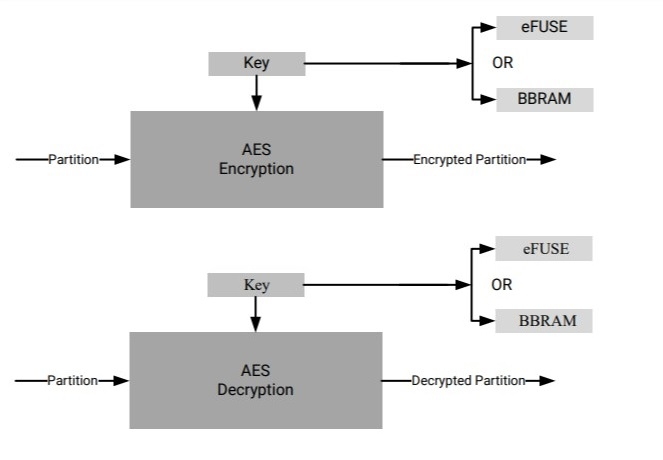
\includegraphics[width=1\textwidth]{imagenes/autentication.jpg}
	\caption{\label{fig1}Cifrado y descifrado de una partición.}
\end{figure}


Este procedimiento es el seguido para un entorno de producción. En el caso de un entorno de desarrollo se utiliza una técnica distinta que consiste en insertar la clave pública en la cabecera del código de arranque (Boot Header) en lugar de en los registros OTP. Para utilizar esta técnica, es necesario incluir una serie de atributos al fichero BIF (Boot Information File) utilizado para crear el binario de arranque (\textit{boot.bin}) \cite{bootgen}. Desafortunadamente dichos atributos solamente son soportados para dispositivos Zynq UltraScale+ MPSoC, entre los cuales no se encuentra la Zedboard. \newline

Al mismo tiempo que se encuentra este problema se descubre el proyecto OP-TEE. Dicho proyecto realiza tanto la parte relacionada con TrustZone como la autenticación de manera automática. La integración de dicho proyecto supone un gran paso con el único inconveniente del cambio de Zedboard a Raspberry Pi 3.



\section{ARM TrustZone en Raspberry Pi 3}

